\chapter{Supporting Information: The transition from invasion to
  persistence for influenza antigenic units}


%\title{Introducing gradual antigenic drift in co-circulating
%  cross-reactive antigenic clusters models}

%other title proposals
%\title{Chaotic dynamics with uniform phase in influenza
%  epidemics: from theory to observation}


Sébastien Ballesteros$^{1,*}$,
Anton Camacho$^{1}$,
Elisabeta Vergu$^{2}$,
Bernard Cazelles$^{1,3}$

\tikzstyle{naif} = [draw, fill=white, rectangle, minimum height=2em, minimum width=3em]
\tikzstyle{expo} = [draw, fill=blue, circle,minimum height=2em]
\tikzstyle{mut} = [draw, fill=red, circle,minimum height=2em]

\definecolor{monVert}{RGB}{120,212,144}
\tikzstyle{class_X} = [draw, fill=blue!20, rectangle, minimum height=2em, minimum width=3em]
\tikzstyle{class_X_2} = [draw, fill=monVert, rectangle, minimum height=2em, minimum width=3em]
\tikzstyle{class_X_3} = [draw, fill=red!20, rectangle, minimum height=2em, minimum width=3em]

\tikzstyle{class_I} = [draw, fill=blue!20, circle,minimum height=2em]
\tikzstyle{class_I_2} = [draw, fill=monVert, circle,minimum height=2em]



\vspace{2cm}

$^1$UMR 7625  (UPMC, ENS, AgroParisTech, CNRS), Ecole Normale Supérieure, Unit of Eco-Evolutionary Mathematics,  46 rue d'Ulm, F-75230 Paris Cedex 05, France. \\
$^2$~INRA, UR341 Mathématiques et Informatique Appliquées, F-78352 Jouy en Josas, France \\
$^3$~IRD UR GEODES, 93142 Bondy, France

~\\
$^*$\textit{Corresponding author}:  \\
E-mail: sebastien.ballesteros@biologie.ens.fr



\section{Justification of the $SIRX$ model}

Here we justify the use of the two levels $SIRX$ model.  We first
introduce single level history based model, and then consider status
based model as the choice of a given framework can have important
consequences on both transient \citep{Ballesteros2009} and stationary
\citep{Dawes2002} dynamics.

\subsection{History based models}

Using the $SIRS$ description of antigenic drift \citep{Pease1987}, we
can incorporate gradual antigenic drift into a two IAU model starting
from simple two strains $SIR$ models and adding loss of immunity
induced by viral evolution (figure~\ref{fig:drawbacks}).

\begin{figure}[h!]
  \center
%%%%%%%%%%%%%%%%%%%%%%%%%%%%%%%%%%%%%%%%%%%%%%%%%%%%%%%%%%%%%%%%%%%%%%%%%
% naive status based model (reduced susceptibility)
%%%%%%%%%%%%%%%%%%%%%%%%%%%%%%%%%%%%%%%%%%%%%%%%%%%%%%%%%%%%%%%%%%%%%%%%%
\begin{minipage}{0.45\linewidth}
  \begin{tikzpicture}[node distance=1.4cm, inner sep=0pt, minimum size=8mm]
    \tikzstyle{seb}=[rectangle, fill=red, draw=gray, text=black]
    \tikzstyle{I1}=[->, draw=red, shorten >=1pt, >=stealth',semithick]
    \tikzstyle{I2}=[->,draw=blue, shorten >=1pt, >=stealth',semithick]
    \tikzstyle{g1}=[->,shorten >=1pt, >=stealth',semithick]
    \tikzstyle{g2}=[->,shorten >=1pt, >=stealth',semithick]

    \node[seb] (R0) {$R_\varnothing$};
    \node[seb] (R1) [above of=R0] {$R_1$};
    \node[seb] (R2) [below of=R0] {$R_2$};
    \node[seb] (R12) [right of=R0] {$R_{12}$};

    \draw[I1] (R0) to node[auto] {\begin{tiny}$(1-\sigma'_{12}) \beta R_\varnothing I^1$\end{tiny}} (R1);
    \draw[I2] (R0) to node[auto,swap] {\begin{tiny}$(1-\sigma'_{12}) \beta R_\varnothing I^2$\end{tiny}} (R2);
    \draw[I2] ([yshift=+4mm] R1.east) to node[auto] {\begin{tiny}$\beta R_1 I^2$\end{tiny}} ([yshift=+4mm] R12.west);
    \draw[I1] ([yshift=-4mm] R2.east) to node[auto,swap] {\begin{tiny}$\beta R_2 I^1$\end{tiny}} ([yshift=-4mm] R12.west);
    \draw[g1] ([xshift=+2mm] R1.south) to node[auto] {\begin{tiny}$\gamma_1 \gamma_2$\end{tiny}} ([xshift=+2mm] R0.north);
    \draw[g2] ([xshift=+2mm] R2.north) to node[auto,swap] {\begin{tiny}$\gamma_2 \gamma_1$\end{tiny}} ([xshift=+2mm] R0.south);
    \draw[g1] (R12.west) to (R2.east) ;
    \draw[g2] (R12.west) to (R1.east) ;
    \draw[I1] ([yshift=+1mm] R0.east) to node[auto] {\begin{tiny}$\sigma'_{12} \beta R_\varnothing I^1$\end{tiny}} ([yshift=+1mm] R12.west);
    \draw[I2] ([yshift=-1mm] R0.east) to node[auto,swap] {\begin{tiny}$\sigma'_{12} \beta R_\varnothing I^2$\end{tiny}} ([yshift=-1mm] R12.west);
\end{tikzpicture}
\end{minipage}
%%%%%%%%%%%%%%%%%%%%%%%%%%%%%%%%%%%%%%%%%%%%%%%%%%%%%%%%%%%%%%%%%%%%%%%%%
% naive history based model (reduced susceptibility)
%%%%%%%%%%%%%%%%%%%%%%%%%%%%%%%%%%%%%%%%%%%%%%%%%%%%%%%%%%%%%%%%%%%%%%%%%
\begin{minipage}{0.45\linewidth}
  \begin{tikzpicture}[node distance=1.4cm, inner sep=0pt, minimum size=8mm]
    \tikzstyle{seb}=[rectangle, fill=red, draw=gray, text=black]
    \tikzstyle{I1}=[->, draw=red, shorten >=1pt, >=stealth',semithick]
    \tikzstyle{I2}=[->,draw=blue, shorten >=1pt, >=stealth',semithick]
    \tikzstyle{g1}=[->,shorten >=1pt, >=stealth',semithick]
    \tikzstyle{g2}=[->,shorten >=1pt, >=stealth',semithick]

    \node[seb] (R0) {$R_\varnothing$}; 
    \node[seb] (R1) [above of=R0] {$R_1$};
    \node[seb] (R2) [below of=R0] {$R_2$};
    \node[seb] (R12) [right of=R0] {$R_{12}$};

    \draw[I1] (R0) to node[auto] {\begin{tiny}$\beta R_\varnothing I^1$\end{tiny}} (R1);
    \draw[I2] (R0) to node[auto,swap] {\begin{tiny}$\beta R_\varnothing I^2$\end{tiny}} (R2);
    \draw[I2] ([yshift=+4mm] R1.east) to node[auto] {\begin{tiny}$\sigma_{12} \beta R_1 I^2$\end{tiny}} ([yshift=+4mm] R12.west); 
    \draw[I1] ([yshift=-4mm] R2.east) to node[auto,swap] {\begin{tiny}$\sigma_{12} \beta R_2 I^1$\end{tiny}} ([yshift=-4mm] R12.west);
    \draw[g1] ([xshift=+2mm] R1.south) to node[auto] {\begin{tiny}$\gamma_1 \gamma_2$\end{tiny}} ([xshift=+2mm] R0.north); 
    \draw[g2] ([xshift=+2mm] R2.north) to node[auto,swap] {\begin{tiny}$\gamma_2 \gamma_1$\end{tiny}} ([xshift=+2mm] R0.south) ;
    \draw[g1] (R12.west) to (R2.east) ;
    \draw[g2] (R12.west) to (R1.east) ;
  \end{tikzpicture}
\end{minipage}
\caption{Drawbacks of introducing antigenic drift in simple status
  based (left) and history based (right) two strains (here IAU) models
  (reduced susceptibility assumption). Red (blue) arrows represent
  infection by IAU 1 (2). Black arrows represent within IAU antigenic
  evolution.}
\label{fig:drawbacks}
\end{figure}

In a history based model with reduced susceptibility
(figure~\ref{fig:drawbacks}, right ; eq~\eqref{eq:appendix3:HBRS}),
infection of hosts naive to both IAU $i$ and $j$ ($R_\varnothing$)
with IAU $i$ results in all infected hosts acquiring immunity to $i$
($R_\varnothing \rightarrow R_i$) and a partial protection to $j$ that
will be determined at the encounter time with $j$. As IAU $i$ evolves,
the population looses immunity to IAU $i$.

This processes can be formalised by extending multi strain model of
\cite{Andreasen1997} to include gradual antigenic drift within IAU
(eq~\eqref{eq:appendix3:HBRS}) (note that we also allow coinfections)

%HBRS 1 level coinfections
\begin{align}
  \label{eq:appendix3:HBRS}
  \dot{R_\varnothing} &= \mu N -\sum_k \beta_k R_\varnothing \frac{I^k}{N} +\sum_{k \in K} g_k
  R_k - \mu R_\varnothing\\
  %% 
  \dot{R_J} &= \sum_{k \in J} \beta_k {\sigma}^k_{J \setminus k} R_{J
    \setminus k} \frac{I^k}{N} - \sum_{k \notin J} \beta_k {\sigma}^k_J R_J \frac{I^k}{N} -
  \sum_{k \in J} g_k R_J + \sum_{k \notin J} g_k
  R_{J \cup k} -\mu R_J \notag \\
  %% 
  \dot{I^k} &= \sum_{J \subseteq \{K \setminus k\}} {\sigma}^k_J \beta_k
  R_J \frac{I^k}{N} -\nu I^k -\mu I^k \notag
\end{align}

where $J$ denotes the set of all previous IAU (belonging to the set
$K$) that have successfully infected and immunised the hosts.

At the single IAU level, model of eq \eqref{eq:appendix3:HBRS} is
reduced to the classical $SIRS$ model. The addition of gradual
antigenic drift increases the proportion of infectious hosts at the
endemic equilibrium compared to the $SIR$ model resulting in:
$I_{SIRS}^*=\frac{e+\gamma}{1+\gamma} (1-\frac{1}{r}) =I_{SIR}^* +
\frac{\gamma}{1+\gamma}R_{SIR}^*$. The number of susceptible
individuals ($R_\varnothing$) however remains the same as for the
$SIR$ model with an equilibrium value of $1/r$.  In the absence of
functional constraints, this condition renders the invasion of a
second IAU always possible in a population where a resident IAU is at
the endemic equilibrium.


One of the major drawbacks of the multi IAU $SIRS$ model ($muSIRS$) is
that if IAU $i$ evolves we loose the fact that $R_i$ hosts (now
$R_\varnothing$) are partially protected to the second IAU. This
assumption would be relevant for waning immunity but in our case
contradicts the fact that influenza specific immune response appears
to be long-lived. The memory of partial protection is important to
take into account as the IAU can be considered separated by a fixed
antigenic distance that remains constant despite within IAU evolution
\citep{Blackburne2008}. Only punctual events create new IAU.


Keeping track of partial cross protection despite within IAU gradual
antigenic drift is possible by introducing a new compartment $X$
(figure \ref{fig:sirx}).

\begin{figure}[H]
\center
  \begin{tikzpicture}[node distance=2cm, auto,>=latex', thick]
    \tikzstyle{seb}=[->,draw=red, shorten >=1pt, >=stealth',semithick]
    % We need to set at bounding box first. Otherwise the diagram
    % will change position for each frame.
    % \path[use as bounding box] (-1,0) rectangle (10,-2);
    \node [naif] (S) {$S$};
    \node [expo, right of=S] (I) {$I$};
    \node [expo, right of=I] (R) {$R$};
    \node [expo, right of=R] (X) {$X$};
    \node [mut, below of=I] (I2) {$I_2$};
    % \node [mut, below of=R] (I2) {$I_2$};
    % \node [mut, below of=X] (I2) {$I_2$};
    
    % Once the nodes are placed, connecting them is easy. 
    \draw [->] (S) -- node {$r$} (I);
    \draw [->] (I) -- node{$(1-e)$}(R);
    \draw [->] (R) -- node{$\gamma$}(X);
    \draw[seb, ->](X) -- +(0,1) -| node[near start,above] {$\sigma_X r$} (I);
    \draw [->] (S) -- node {$\alpha r$} (I2);
    \draw [->] (I) -- node {$\sigma_{12} \alpha r$} (I2);
    \draw [->] (R) -- node {$\sigma_{12} \alpha r$} (I2);
    \draw [seb, ->] (X) -- node {$\sigma_{12} \alpha r$} (I2);    
  \end{tikzpicture}
  \caption{The $SIRX$ model: new-borne ($S$) have full susceptibility,
    within IAU antigenic evolution results in the loss of full
    immunity toward strain of the IAU ($R \to X$). $X$ host can
    retain a level of partial protection to reinfection
    ($\sigma_X$). Hetero unit partial protection is ensured by
    parameter $\sigma_{12}$.}
\label{fig:sirx}
\end{figure}

This is the model used in main text.

Keeping track of partial protection despite within IAU antigenic
evolution have important consequences on the invasion condition of a
mutant IAU. Here we generalise the invasion threshold presented in
main text to a population where $K$ identical unrelated (and therefore
non cross reactive) resident IAU are at the endemic equilibrium. This
condition can be calculated with
 $$\left. \frac{d I^{K+1}}{d t} \right|_{1^*,\dots, K^*} =
(r_{K+1} R_{\begin{subarray}{l}\varnothing \\
    \varnothing \end{subarray}}^* + \sigma_{12} r_{K+1}
(1-R_{\begin{subarray}{l}\varnothing \\ \varnothing \end{subarray}}^*)
-1) I^{K+1}$$
where we use non dimensional form of the models by
rescaling natural time $t$ in unit of duration of infection and note
$r=\frac{\beta}{\mu+\nu}$, $e=\frac{\mu}{\mu+\nu}$;
$\gamma=\frac{g}{\mu+\nu}$.

In the following, we assume that $r_{K+1}=\alpha r$ and expect $\alpha
\leq 1$ due to functional constraints.

The invasion condition can be expressed as $\sigma_{12} > \frac{1-\alpha
  r R_{\begin{subarray}{l}\varnothing \\
      \varnothing \end{subarray}}^*}{\alpha
  r(1-R_{\begin{subarray}{l}\varnothing \\
      \varnothing \end{subarray}}^*)}$ and is determined only by
$R_{\begin{subarray}{l}\varnothing \\ \varnothing \end{subarray}}^*$


This expression is also valid for the $muSIRS$ model. For this latter
model, when $K=1$, the number of fully naive hosts is given by
$1/r$. In the absence of functional constraints ($\alpha=1$) fully
naive hosts are always in a sufficient number to ensure the invasion
of a mutant IAU ($1-r R_{\begin{subarray}{l}\varnothing \\
    \varnothing \end{subarray}}^*=0$) and there is no invasion
threshold.  Situation changes with the $SIRX$ model or when $K>1$
unrelated IAU co-circulate. In these cases,
$R_{\begin{subarray}{l}\varnothing \\ \varnothing \end{subarray}}^*$
can be calculated from: $\frac{dR_{\begin{subarray}{l}\varnothing \\
      \varnothing \end{subarray}}^*}{dt} = 0 = e -r
R_{\begin{subarray}{l}\varnothing \\ \varnothing \end{subarray}}
\sum_kI^k -e
R_{\begin{subarray}{l}\varnothing \\ \varnothing \end{subarray}}$.\\

As there is no competition at all in the resident population, the
endemic equilibrium of IAU $k \in [1,\dots,K]$, ${I^k}^*$ are all
identical to the value $I^*$ of the single IAU model.  The invasion
condition can then be expressed as a function of $I^*$:
$\sigma_{12}>\frac{KrI^*+e(1-\alpha r)}{K \alpha r^2 I^*}$.  In the
special cases where $\sigma_X=1$ an exact expression can be derived as
$I^*$ is given by the equilibrium of the simple $SIRS$ model.

\begin{align}
  \label{eq:appendix3:threshold}
  \sigma_{12} &> \frac{1}{\alpha r} - \frac{e(1+\gamma)(\alpha r-1)}{K
    \alpha r (e+\gamma)(r-1)}
\end{align}

In this latter case, gradual antigenic drift within IAU $g>0$ ensures
an invasion threshold even when $K=1$ and $\alpha=1$.  and possesses
an upper bound $=\frac{1}{r} - \frac{e}{K r}$ as $\gamma \to \infty$.

As we show in main text, the invasion of a mutant IAU is always
possible whenever $\sigma_{12} > \sigma_X$.

This sufficient condition is not limited to the simple $SIRX$ model
and remains valid for models allowing a flexible shape of the
evolution of the reinfection probability following antigenic drift
such the one used by \citet{Xia2005}.


The model depicted in figure~\ref{fig:general} allow to consider
flexible shape of the evolution of the reinfection probability
following antigenic drift.  Note that as hosts never come back to the
$S$ compartment, we ensure that hosts partially protected to a new IAU
keep their partial protection even if the originally immunising IAU is
subject to antigenic drift rendering reinfection by the same IAU
possible.  The flexibility of this model was used by \cite{Xia2005} to
infer the shape of the immunity decay following influenza infection.
$(1-\sigma_{12})$ is the reduction of susceptibility due to inter-IAU
partial cross protection and $(1-\sigma_X)$ is the the reduction of
susceptibility due to within-IAU partial cross protection.

\begin{figure}[h!]
\center
\begin{tikzpicture}[node distance=2cm, auto,>=latex', thick]
  \tikzstyle{seb}=[->,draw=red, shorten >=1pt, >=stealth',semithick]
    % We need to set at bounding box first. Otherwise the diagram
    % will change position for each frame.
%    \path[use as bounding box] (-1,0) rectangle (10,-2);
    \node [naif] (S) {$S$};
    \node [expo, right of=S] (I) {$I$};
    \node [expo, right of=I] (R1) {$R_1$};
    \node [expo, right of=R1] (R2) {$R_2$};
    \node [expo, right of=R2] (Rk) {$R_K$};
    \node [mut, below of=I] (I2) {$I_2$};

% Once the nodes are placed, connecting them is easy. 
    \draw [->] (S) -- node {$r$} (I);
    \draw [->] (I) -- node{$(1-e)$}(R1);
    \draw [->] (R1) -- node{$K \gamma$}(R2);
    \draw [->] (R2) -- node{...}(Rk);
    \draw[->](R1) -- +(0,1) -| node[near start,above] {$\sigma_X^1 r$}
    (I);
    \draw[->](R2) -- +(0,1.7) -| node[near start,above] {$\sigma_X^2 r$}
    (I);
    \draw[->](Rk) -- +(0,2.4) -| node[near start,above] {$\sigma_X^K r$}
    (I);

    \draw [seb, ->] (S) -- node {$\alpha r$} (I2);
    \draw [seb, ->] (I) -- node {$\sigma_{12} \alpha r$} (I2);
    \draw [seb, ->] (R1) -- node {$\sigma^1_{12} \alpha r$} (I2);
    \draw [seb, ->] (R2) -- node {$\sigma^2_{12} \alpha r$} (I2);
    \draw [seb, ->] (Rk) -- node {$\sigma^K_{12} \alpha r$} (I2);
    
\end{tikzpicture}
\caption{A general model for a drifting antigenic unit.}
\label{fig:general}
\end{figure}

Using figure~\ref{fig:general} model, the invasion condition of a
second IAU can be calculated with:\\
$\left. \frac{d I^2}{d t} \right|_{1^*} = (\alpha r S^* + \alpha r (
\sum_k \sigma^k_{12} R_k^* + \sigma_{12} I) -1) I^2 >0$.

Assuming that the first IAU is at the epidemiological equilibrium
ensures that: $\frac{dI}{dt} = r S I +r \sum_k \sigma_X^k R_k I -I = 0
\Rightarrow r S^* + r \sum_k \sigma_X^k R_k^*=1$

Considering $\alpha=1$, invasion is always possible if $\sum_k
\sigma^k_{12} R_k^* > \sum_k \sigma_X^k R_k^*$. This condition is always
true if $\forall{k} \in [1, ..., K]$, $\sigma^k_{12} > \sigma_X^k$. Note
that in the absence of co-infections, this condition also defines the
invasion threshold.

$\sigma^k_{12} > \sigma_X^k$, $\forall{k} \in [1, ..., K]$, therefore
constitutes a sufficient condition for the invasion of the mutant
IAU.





\subsection{Status based model}


%SBRI---------------

Within a status based framework (figure~\ref{fig:drawbacks}, left),
following infection with IAU $i$, naive hosts acquire immunity to $i$
($R_i$) and a given proportion ($\sigma'_{12}=1-\sigma_{12}$) acquires
immunity to both $i$ and $j$ ($R_{ij}$) and are therefore no more
susceptible for both IAUs $i$ and $j$ (polarized immunity
\citet{Gog2002a}).  We can thus easily take into account the fact that
IAU $i$ can evolve and thus the population looses immunity to cluster
$i$ but not to cluster $j$. This results in a $R_{ij} \rightarrow R_j$
transfer.

Contrary to history based model, assuming that cross-immunity acts by
reducing susceptibility or infectivity have strong consequecences on
status based model \citep{Ballesteros2009}.  All the theoretical
studies supporting the punctuated theory of influenza immune escape
have used the reduced infectivity formalism ($SBRI$ model) as it
results in comparatively low dimensional models.  The $SBRI$ model
including within IAU gradual antigenic drift is depicted in
eq~\eqref{eq:SBRI} where $S_k$ denotes hosts susceptible to IAU $k$.

%SBRI
\begin{footnotesize}
  \begin{align}
    \label{eq:SBRI}
    \dot{S_k} &= \mu N -\sum_j \beta_j(t) {\sigma'}_{kj} S_k
    \frac{I^j}{N}
    - \mu S_k +g_k (N-S_k-I^k)\\
  %% 
    \dot{I^k} &= \beta_k S_k \frac{I^k}{N} -\nu I^k -\mu I^k \notag
  \end{align}
\end{footnotesize}

In case of reduced susceptibility assumption ($SBRS$ model), including
within IAU gradual antigenic drift results in eq~\eqref{eq:SBRS}.

\begin{footnotesize}
  \begin{align}
    \label{eq:SBRS}
    \dot{R_\varnothing} &= \mu N -\sum_k \beta_k R_\varnothing
    \frac{I^k}{N} +\sum_{k \in K} g_k
    R_k - \mu R_\varnothing\\
  %% 
    \dot{R_J} &= \sum_{k, L \subseteq K} C(L,J,k) \beta_k
    \frac{I^k}{N} R_L -\sum_{k \in \{J \setminus k\}} \beta_k
    \frac{I^k}{N} R_J -\sum_{k \in J} g_k R_J + \sum_{k \notin J} g_k
    R_{J \cup k} -\mu R_J \notag \\
  %% 
    \dot{I^k} &= \sum_{J \subseteq \{K \setminus k\}} \beta_k R_J
    \frac{I^k}{N} -\nu I^k -\mu I^k \notag
  \end{align}
\end{footnotesize}

where following \citet{Gog2002a}, 

$$C(L,J,k)=
\begin{cases}
  \prod_{j \in J \setminus L} \sigma'_{kj} \prod_{j \notin J}
  (1-\sigma'_{kj}) & \text{if } k \notin L \text{ and } L \subset J \\
  0 & \text{otherwise.}
\end{cases}$$


As shown in figure \ref{SBRI_2}, the status-based formulation induces
an immune boosting dynamics that can be illustrated in the 2-IAUs
case. When IAU $2$ has yet not appeared and thus does not evolve (no
gradual antigenic drift for $2$), figure \ref{SBRI_2} shows that, in
the absence of birth, $R_{2}+R_{12}$ form an absorbing class. The
infection dynamics of strain $1$ rapidly results in an equilibrium
mostly governed by a reinfection dynamics between $R_2$ and
$R_{12}$. This process results in the fact that when cluster $2$
appears, it cannot invade as all the hosts have full immunity to
$2$. Moreover, with the assumption of reduced infectivity, the $SBRI$
model leads to a transfer $R_{1}\to R_{12}$ (in red on figure
\ref{SBRI_2}) that overestimates the immunity against IAU 2. From a
biological stand point, this additional transfer resulting from
reinfection of $R_1$ by IAU 1 is even more problematic as it is in
disagreement with the original antigenic sin mechanism
\citep{Ballesteros2009}.

\begin{center}
\begin{figure}[h!]
\centering
\begin{tikzpicture}[node distance=3cm, auto,>=latex', thick]

  \tikzstyle{output} = [coordinate]
  
  \node [class_X] (R0) {$R_{\emptyset}$};	
  
  \node [class_X_3, right of=R0,node distance=5cm] (R12) {$R_{12}$};
  
  \draw [->] (R0) --node[name=R0R12] {$\sigma'_{12}\lambda_1$}(R12);
  
  \node [class_X_2, above of=R0R12,node distance=2cm] (R1) {$R_1$};
  \node [class_X_2, below of=R0R12,node distance=2.5cm] (R2) {$R_2$};
  
  \draw [->] (R0) edge[bend left]node[left]{$(1-\sigma'_{12})\lambda_1$}(R1);
  \draw [->] (R1) edge[bend left]node[above]{$g_{1}$}(R0);
  
  \draw [->] (R1) edge[bend left]node[right]{$\textcolor{red}{\sigma'_{12}\lambda_1}$}(R12);
  
  \draw [->] (R2) edge[bend right]node[right]{$\lambda_1$}(R12);
  \draw [->] (R12) edge[bend right]node[below]{$g_{1}$}(R2);
  
\end{tikzpicture}
\caption{Schematic representation of the immune boosting induced by
  status-based frameworks. The assumption of reduced infectivity leads
  to an additional transfer $R_{1}\to R_{12}$ (in red). $\lambda_{1}$
  is the infection force of IAU 1. Note that for comparison purpose
  with history based model, the cross-immunity intensity
  $\sigma'_{12}$ can be simply related to the immune escape intensity
  by $\sigma_{12}=1-\sigma'_{12}$.}
\label{SBRI_2}
\end{figure}
\end{center}

\clearpage

More quantitatively, the impeded invasion produced by the status based
framework can be determined by standard invasion analysis. For
instance for the $SBRI$ model of eq.\eqref{eq:SBRI}, the invasion
condition can be calculated by:

\begin{align}
  \left. \frac{d I^2}{d t} \right|_{S_2^*} & =
  (r_2 S_2^* -1) I^2 \label{eq:invasion_sbri}
\end{align}

where $S_2^*$ is determined by the equilibrium of the 2-IAU model with
$I^2=0$.

Invasion of the mutant IAU implies $\left. \frac{d I^2}{d t}
\right|_{S_2^*} \geq 0$ and results in a threshold on $\sigma'_{12}$:
 $$\sigma'_{12} \leq \frac{(r_2-1)(e+\gamma_2)(1+\gamma_1)}{(r_1-1)(e+\gamma_1)}$$.  
 In the following we assume $r_2=r_1$ ($\alpha=1$ no functional
 constraints). If $\gamma_2=0$ until IAU 2 appears there is an
 invasion trheshold. This threshold does not depend on $R_0$ (here,
 $r$) and is represented on figure~\ref{fig:threshold_koelle}. Note
 however that if $\gamma_2=\gamma_1$ before IAU 2 emerges the invasion
 condition is always satisfied.

\begin{figure}[!htbp]
  \center
  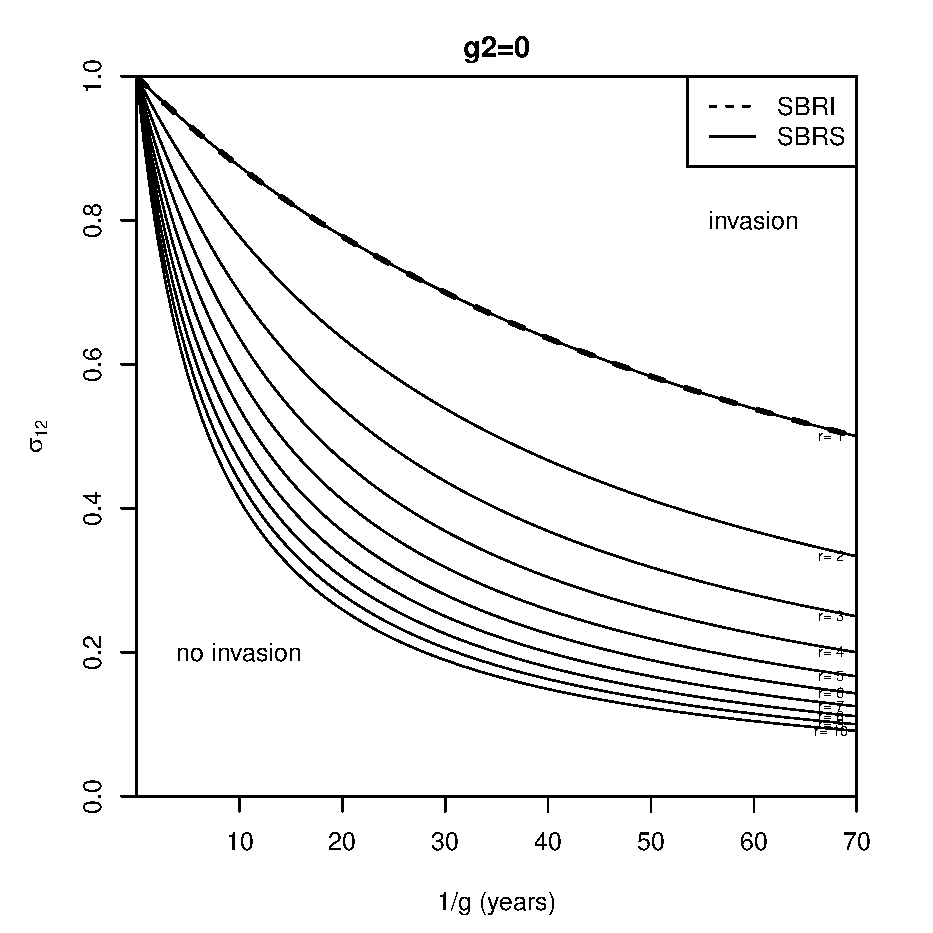
\includegraphics[width=0.3\linewidth]{texte/article3/appendix_diamond/graph/threshold_koelle.eps}
  \caption{Invasion threshold for the two antigenic unit status based
    model ($SBRI$ and $SBRS$) with $r_2=r_1$. Note that for comparison
    purpose with history based model, the y-axis is expressed in
    immune escape intensity with $\sigma_{12}=1-\sigma'_{12}$.}
  \label{fig:threshold_koelle}
\end{figure}

The same results can be established for the $SBRS$ model. The
threshold is given by:
$$\sigma'_{12} \leq \frac{r_1 (r_2-1) (e+\gamma_2)
  (\gamma_2 +r_1(e+\gamma_1)}{(r_1-1)(e+\gamma_1) (\gamma_1 r_1
  +r_2(\gamma_2+e r_1))}$$ and plotted on
figure~\ref{fig:threshold_koelle}.  This threshold depends on $r_{1/2}$
and equal the one of the $SBRI$ model when $r_{1}=r_{2}=1$.

Considering $\gamma_2=\gamma_1$ means that IAUs may evolve
before they have emerged. This hypothesis could be supported if
IAUs co-circulate in a region outside the population area and are
introduced following a source-sink process. However, in the context
of influenza antigenic clusters giving rise to each others, we do not find any biological
motivation.  When $\gamma_2=\gamma_1$, the $SBRS$ model also ensures
invasion of the mutant IAU even if $\sigma_{12}=0$ rendering
immune escape difficult to interpret.

Introducing within IAU gradual antigenic drift in status based
multi-strains models can therefore result in an invasion threshold for
a second IAU. As the same model without gradual antigenic
drift does not present this threshold property \citep{Ballesteros2009},
the impeded invasion comes from the immune boosting dynamics
previously described. Due to this immune boosting dynamics, the timing
of introduction of successive IAUs is of tremendous importance
: if the resident IAU has circulated sufficiently long to
fill in compartments $R_2$ and $R_{12}$ then gradual
antigenic drift will result in a strong invasion threshold for the
next IAU. In contrast, if the mutant IAU appears
sufficiently soon, it will be able to invade. 

\subsection{Comparison of status based and history based framework:
  effect of cross-immune boosting}

In order to examine the influence of the cross-immune boosting
dynamics previously described on the outcome of IAU invasion we
contrast the widely used $SBRI$ model with an equivalent history based
model.  Due to the hypothesis of polarised immunity, the inclusion of
within IAU gradual antigenic drift into status based model results in
full susceptibility of the hosts to within IAU reinfection but do not
cancel partial cross protection against other IAUs.  This assumption
can be translated in the $SIRX$ framework by taking its $SIRS$ limit
($\sigma_{X}=1$) \textit{i.e.} by taking the following matrix of
susceptibility reduction: $\mathbf{\sigma_H^k} = \bordermatrix{ & 1 &
  2\cr 1 & 1 & \sigma_{12} \cr 2 & \sigma_{12} & 1 \cr 12 & 1 & 1 \cr
}$. Contrary to the status based model, the equivalent history based
model does not result in cross immune boosting dynamics whereas both
models reduce to the $SIRS$ model at the single IAU level.

In order to simplify the analysis we will consider the invasion of an
IAU already established and subject to gradual antigenic drift in a
source population but not in our focal population \textit{i.e.}
$g_{1}=g_{2}$. This assumption will ensure equality of mutant and
resident antigenic drift rate and therefore cancel the need to study
the effect of the introduction time of the mutant for the status based
model.

\begin{figure}[!htbp]
  \center
  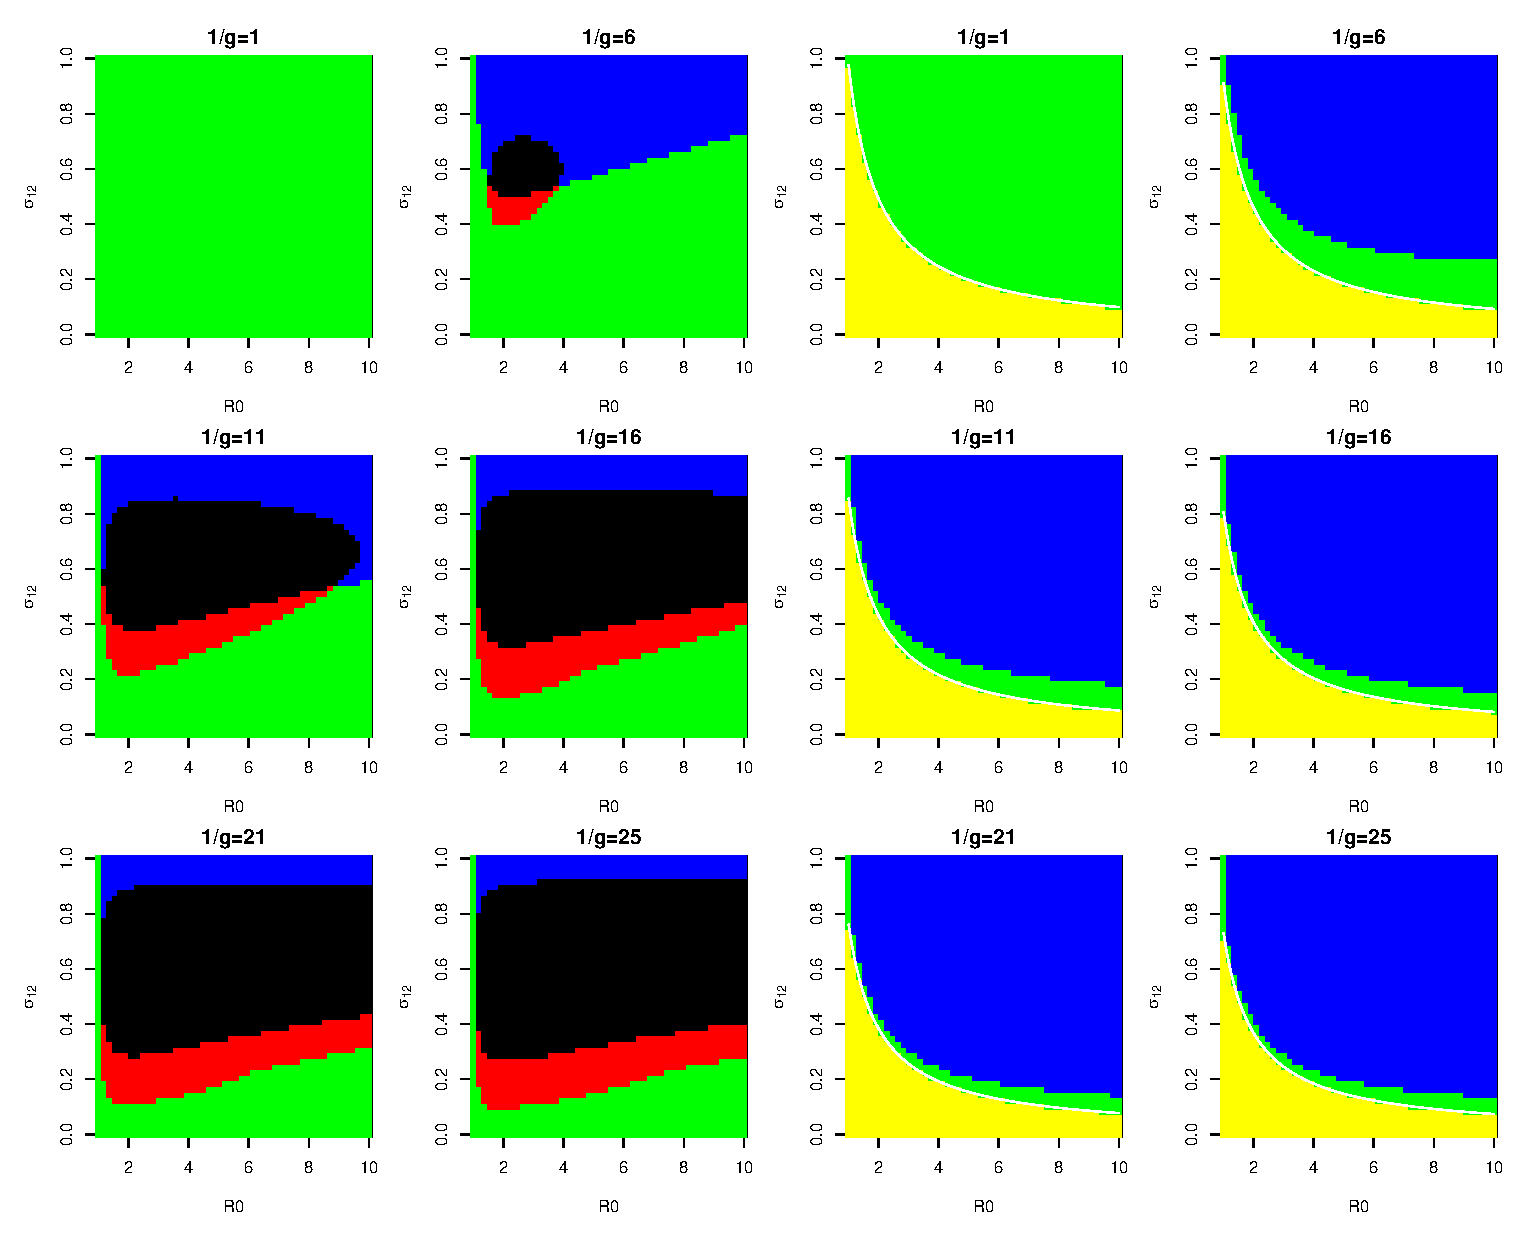
\includegraphics[width=0.8\linewidth]{texte/article3/appendix_diamond/graph/koelle_vs_purely_transiant.eps}
  \caption{Outcomes of the transient invasion dynamics of a new
    IAU within a population where a resident IAU
    is at the endemic equilibrium. First and second column figures are for
    the $SBRI$ model generalised to include within IAU
    gradual antigenic drift (with $g_2=g_1$) ; third and fourth
    column figures are for the equivalent history based model. Colours: both
    IAUs go extinct (black), the resident IAU only goes
    extinct (successful replacement, red); the mutant IAU only goes
    extinct (blue); no IAU goes extinct (coexistence, green); the
    mutant IAU cannot invade (yellow). White curve is the invasion
    threshold given by eq.~\eqref{eq:appendix3:threshold}. As a deterministic
    model is used, extinctions are determined by a threshold value of
    $1.10^{-9}.$}
  \label{fig:koelle_vs}
\end{figure}

As it can be seen in figure~\ref{fig:koelle_vs}, the $SBRI$ model has
a tremendous impact on the outcome of the transient dynamics of
drifting IAUs replacement. Within an equivalent model stated within
the $SIRX$ framework, no replacement (red areas in
figure~\ref{fig:koelle_vs}) are possible for parameter values
compatible with influenza. In place of replacement, the $SIRX$ model
gives rise to a sharp transition from coexistence (green areas in
figure~\ref{fig:koelle_vs}) to self extinction without replacement
(blue areas in figure~\ref{fig:koelle_vs}).



\section{Reinfection limits}

The number of compartment (scaling in $3^{N_K}$) of the $SIRX$, the
$SIRXQ1$ and the $SIRXQ12$ with immune boosting model can be reduced
to $2^{N_K}$ by taking the limit $g \to \infty$.

In case of the $SIRX$ model the reinfection limit leads to
\eqref{eq:SIRI}.

\begin{align}
  \label{eq:SIRI}
  \dot{R_\varnothing} &= \mu N -\sum_k \beta_k R_\varnothing \frac{I^k}{N} - \mu R_\varnothing\\
  %% 
  \dot{R_J} &= \sum_{k \in J} \beta_k \sigma^k_{J \setminus k} R_{J
    \setminus k} \frac{I^k}{N} - \sum_{k \notin J} \beta_k \sigma^k_J R_J \frac{I^k}{N} -\mu R_J \notag \\
  %% 
  \dot{I^k} &= \sum_{J \subseteq K} \sigma^k_J \beta_k
  R_J \frac{I^k}{N} -\nu I^k -\mu I^k \notag
\end{align}

This model is comparable to \cite{Goekaydin2007} model with the
difference that \eqref{eq:SIRI} model allows for coinfections.

Taking the limit $g \to \infty$ of the $SIRXQ1/12$ model results in:

\begin{align}
  \label{eq:SIRIQ}
  \dot{R_\varnothing} &= \mu N -\sum_k \beta_k R_\varnothing \frac{I^k}{N} - \mu R_\varnothing\\
  %% 
  \dot{I^k_J} &= \sigma^k_J \beta_k
  R_J \frac{I^k}{N} + \sigma^k_{J \setminus k} \beta_k
  R_{J \setminus k} \frac{I^k}{N} -\nu I^k_J -\mu I^k_J \notag \\
  %% 
  \dot{Q_J} &= \sum_{k \in J} \nu I^k_J -q Q_J -\mu Q_J \notag \\
  %%
  \dot{R_J} &=  q Q_J - \sum_{k} \beta_k \sigma^k_J R_J \frac{I^k}{N} -\mu R_J \notag
\end{align}

in the absence of immune boosting ($SIRXQ1$) and:

\begin{align}
  \label{eq:SIRIQferg}
  \dot{R_\varnothing} &= \mu N -\sum_k \beta_k R_\varnothing \frac{I^k}{N} - \mu R_\varnothing\\
  %% 
  \dot{I^k_J} &= \sigma^k_J \beta_k
  R_J \frac{I^k}{N} + \sigma^k_{J \setminus k} \beta_k
  R_{J \setminus k} \frac{I^k}{N} -\nu I^k_J -\mu I^k_J \notag \\
  %% 
  \dot{Q_J} &= \sum_{k \in J} \nu I^k_J -q Q_J -\mu Q_J \notag \\
  %%
  \dot{R_J} &=  q Q_J + q Q'_J -\sum_{k} \beta_k R_J \frac{I^k}{N} -\mu R_J \notag \\
  %% 
  \dot{Q'^k_J} &= \sum_{k} (1 - \sigma^k_J) \beta_k R_J \frac{I^k}{N}  -q Q'_J -\mu Q'_J \notag
\end{align}

with immune boosting ($SIRXQ12$).

\section{Additional figures}

\subsection{Transient dynamics: determinist models}

\begin{figure}[!hp]
  \center
  \includegraphics[width=0.9\linewidth]{texte/article3/appendix_diamond/graph/traj_deter.eps}
  \caption{Transient invasion dynamics of a mutant antigenic unit in a
    population where a resident antigenic unit is at its endemic
    equilibrium. Red and blue are prevalence of mutant and resident
    antigenic unit in log scale. Colours intensity indicates the
    degree of immune escape as measured by $\Delta\sigma$ (1\%
    (light tones); 5\%, 10\%, 20\% and 30\% (dark tones)). Parameters:
    $R_0=2$; $1/\nu=4$ days ; $1/g=1$ year ; $1/q=6$
    months. Figure~\ref{fig:traj_deter_reinfection} reveals the
    dynamics obtain by taking the limit $g \to \infty$}
  \label{fig:traj_deter}
\end{figure}

\begin{figure}[!hp]
  \center
  \includegraphics[width=0.9\linewidth]{texte/article3/appendix_diamond/graph/traj_deter_reinfection.eps}
  \caption{Replication of figure~\ref{fig:traj_deter} for the
    reinfection limit models ($g \to \infty$).}
  \label{fig:traj_deter_reinfection}
\end{figure}

\begin{figure}[!hp]
  \center
  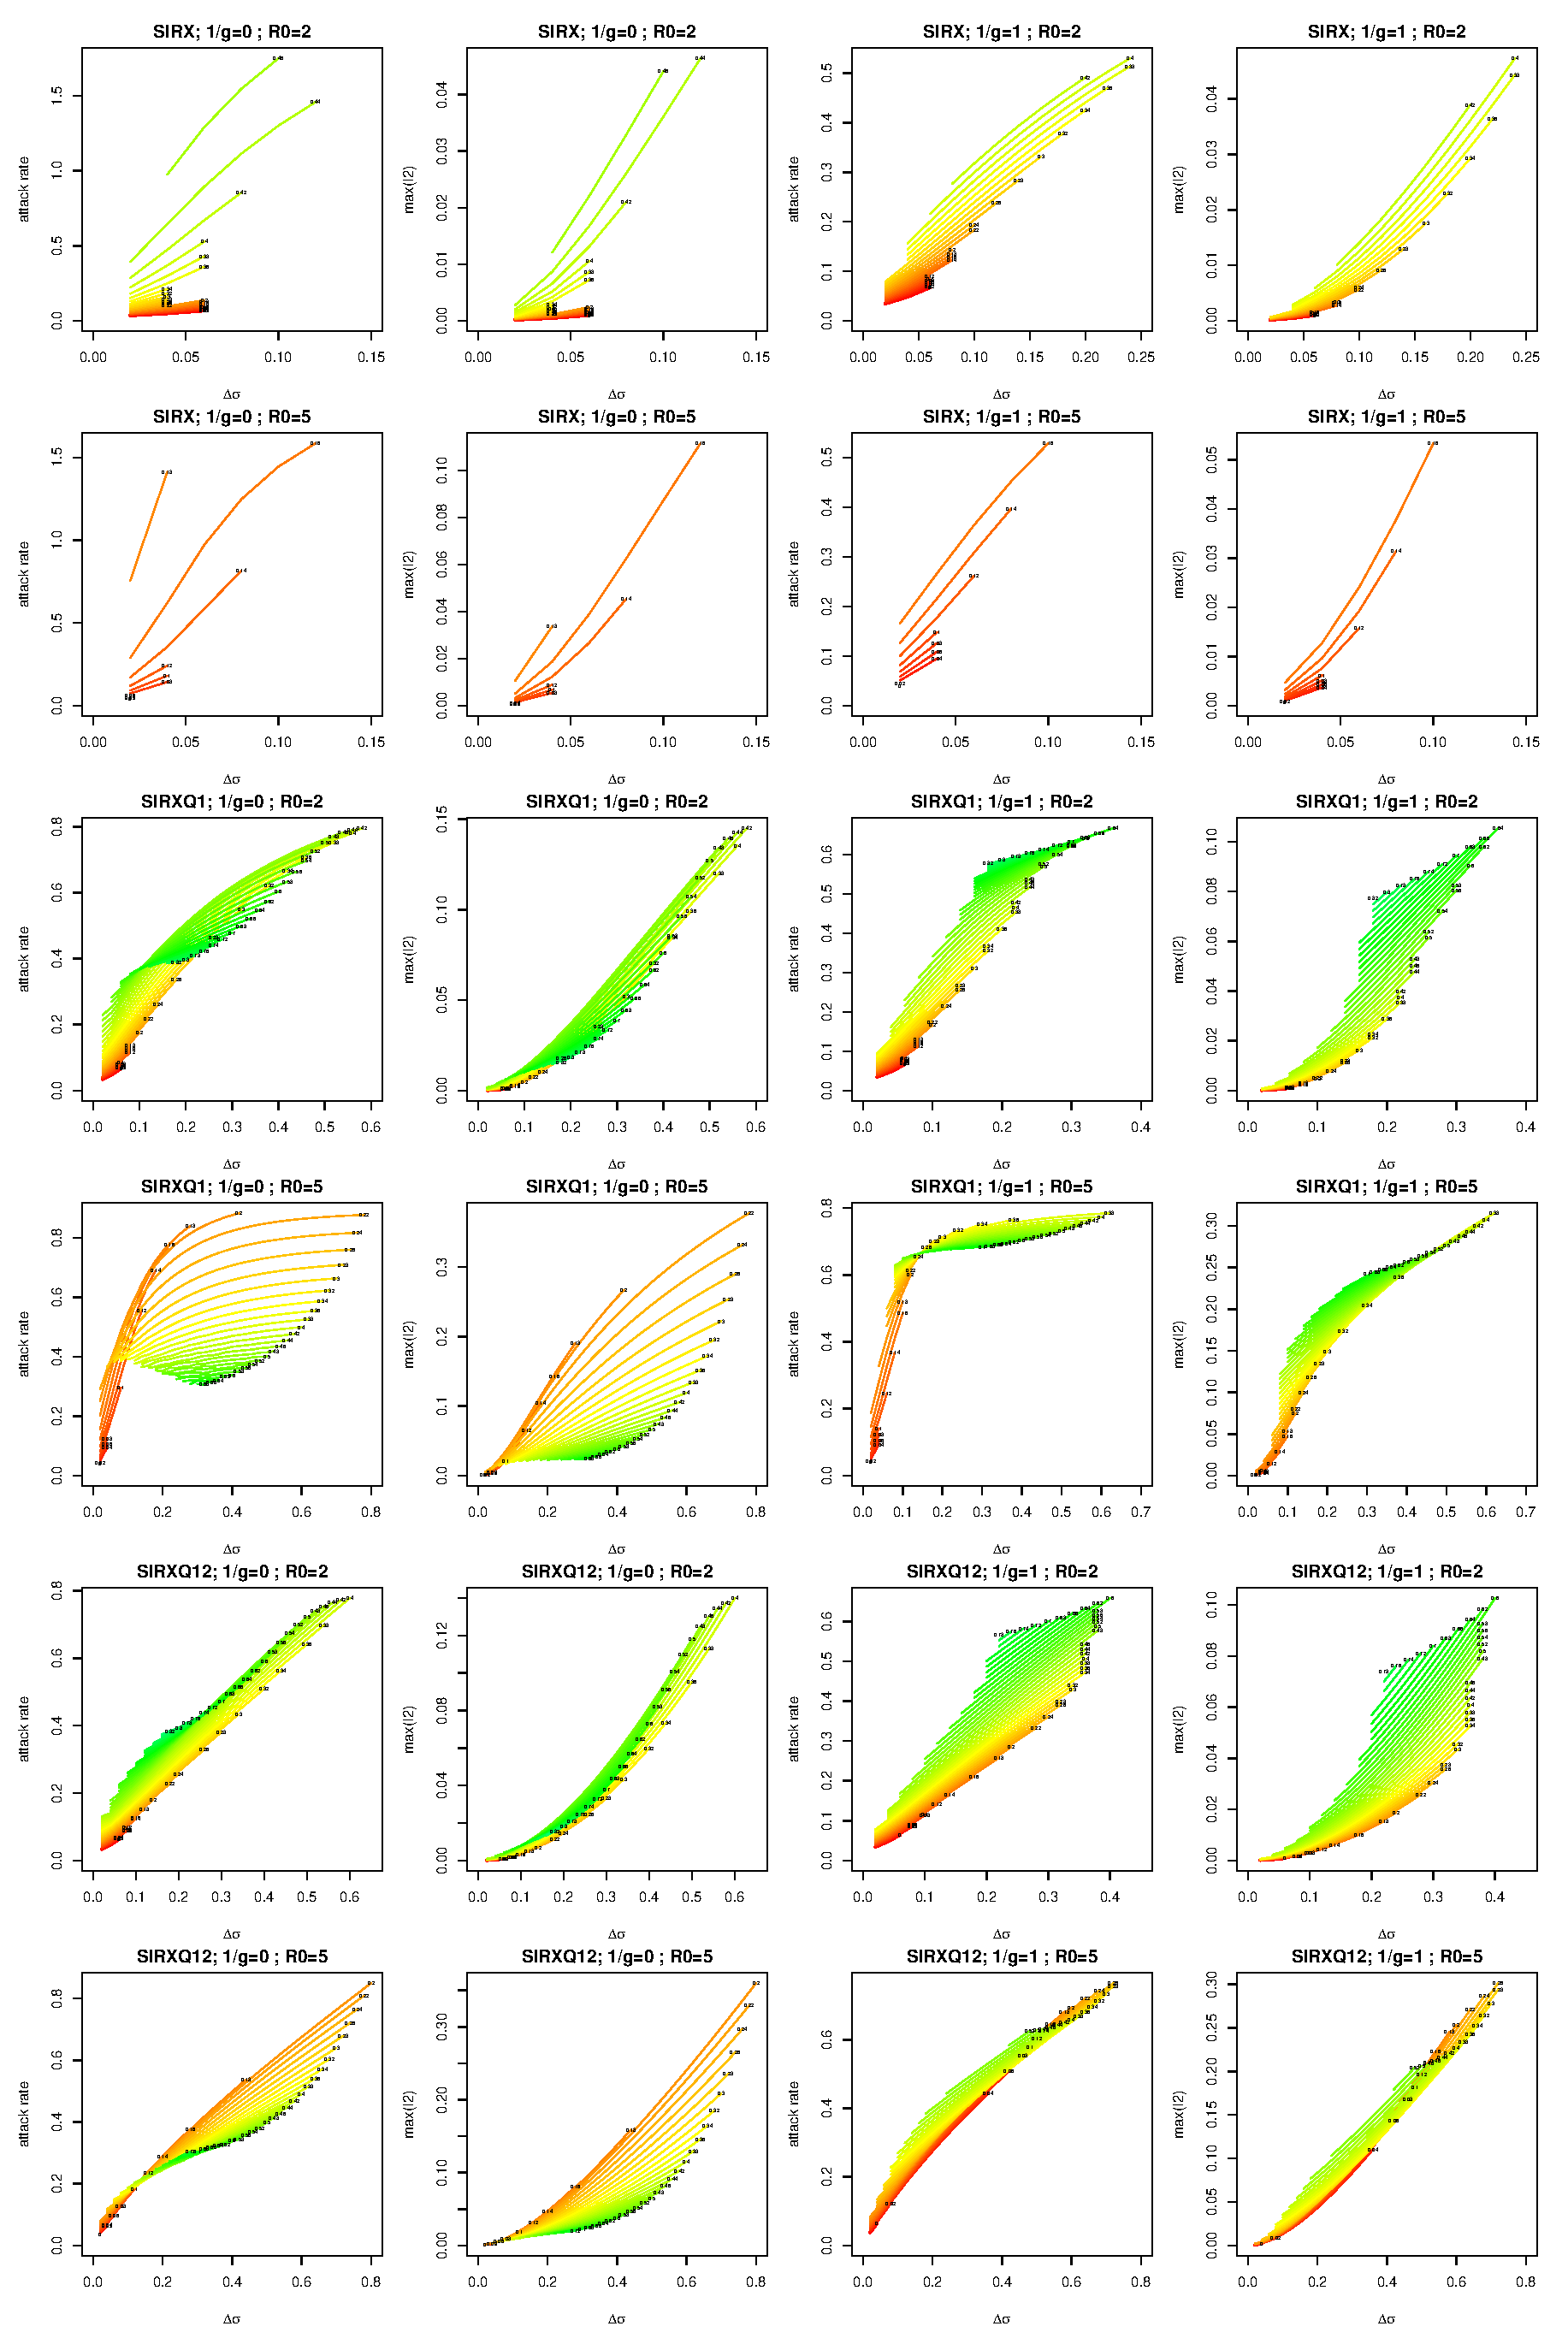
\includegraphics[width=0.8\linewidth]{texte/article3/appendix_diamond/graph/attak.eps}
  \caption{Effect of immune escape on the attack rate and the maximum
    epidemic size of the mutant antigenic unit for the $SIRX$ model
    (first and second lines), the $SIRXQ1$ model (third and fourth
    lines) and the $SIRXQ12$ model with immune boosting (fifth and sixth
    lines) in the parameter space where we expect replacement of the
    resident antigenic unit by the mutant one. Attack rate is
    calculated from the introduction time of the new antigenic unit to
    the first minimum of the epidemic curve. Immune escape is measure
    by $\Delta\sigma$.  Colors represent different values of
    $\sigma_X$ ensuring replacement. Parameters values are identical for
    both antigenic units ($\alpha=1$).}
  \label{fig:sirx_attak}
\end{figure}

\clearpage

\subsection{Effect of functional constraints}


\begin{figure}[!hp]
  \center
  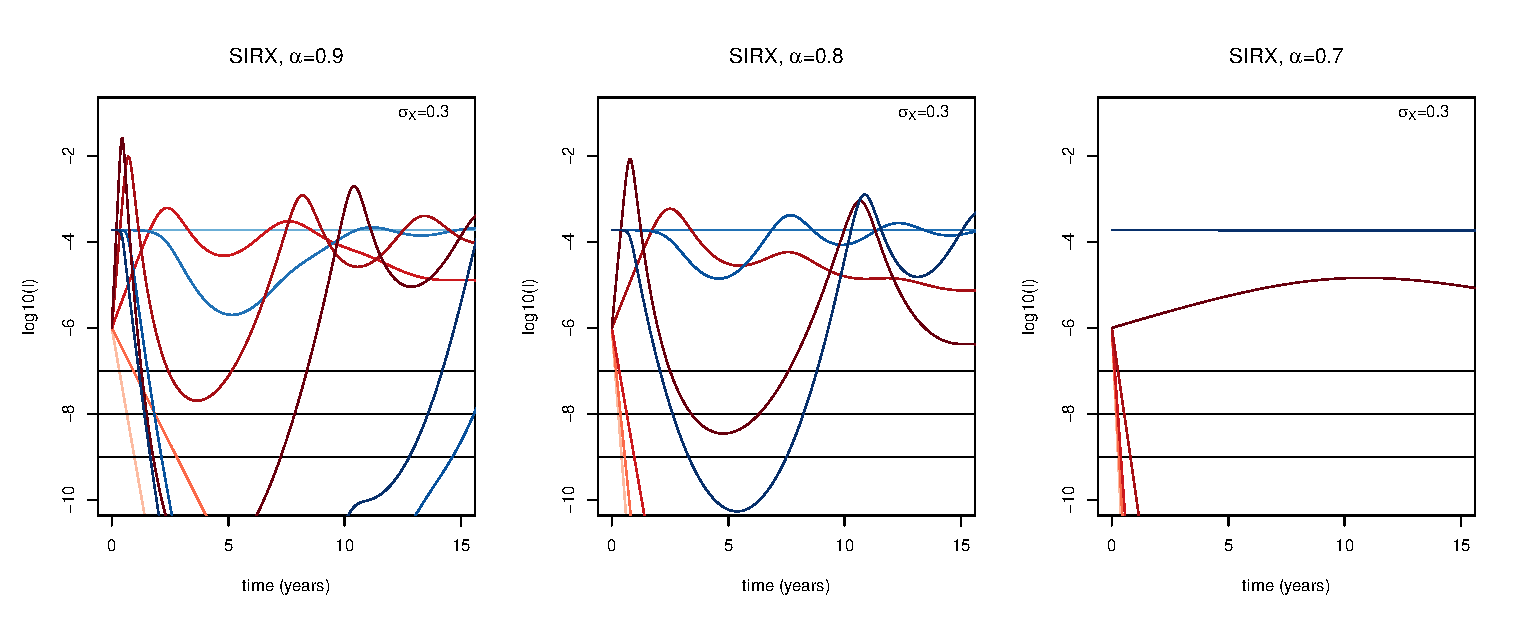
\includegraphics[width=0.9\linewidth]{texte/article3/appendix_diamond/graph/traj_deter_trade_off.eps}
  \caption{Effect of functional constraint on the invasion trajectory
    of a mutant antigenic unit introduced in a population where a
    resident antigenic unit is at the endemic equilibrium for the
    $SIRX$ model. Red and blue are prevalence of mutant and resident
    antigenic unit in log scale. Colours intensity indicates the
    degree of immune escape as measured by $\Delta\sigma$ (1\% (light
    tones); 5\%, 10\%, 20\% and 30\% (dark tones)). Parameters:
    $R_0=2$; $1/\nu=4$ days ; $1/g=1$ year ; $1/q=6$ months}
  \label{fig:traj_deter_trade_off}
\end{figure}

\clearpage

\subsection{Metapopulation dynamics: stochastic models}

\begin{figure}[!hp]
  \center
  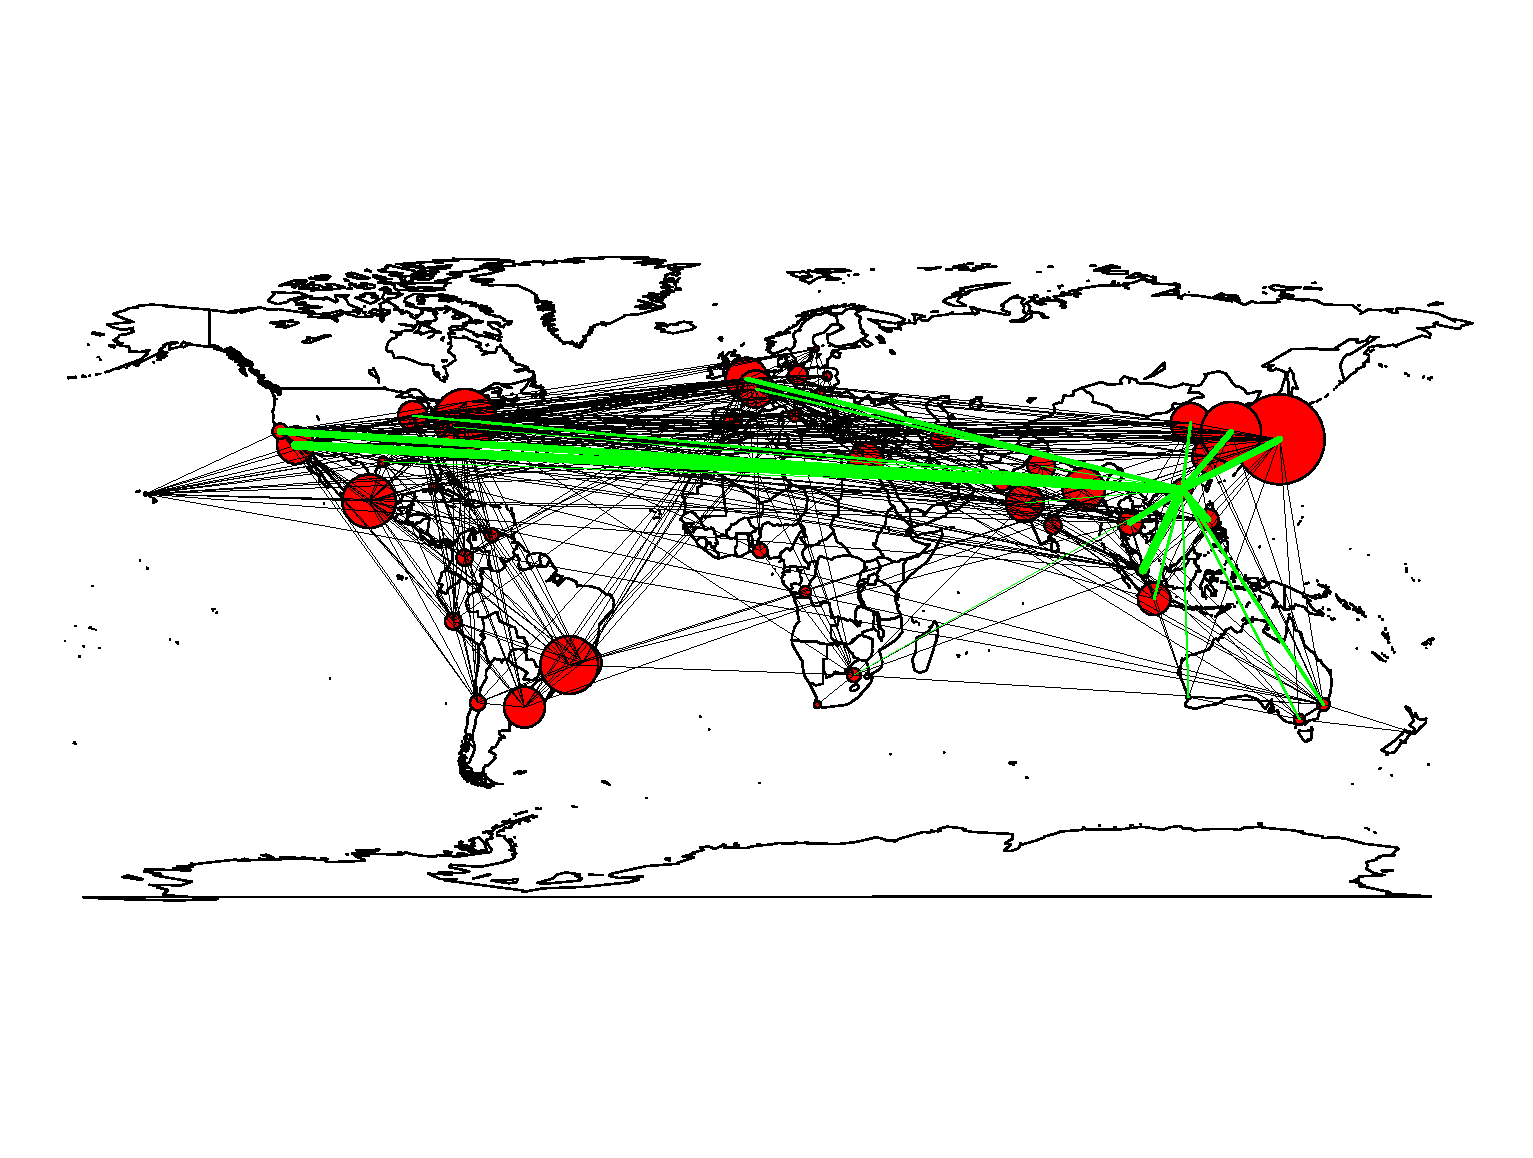
\includegraphics[width=0.6\linewidth]{texte/article3/appendix_diamond/graph/mapHK.eps}
  \caption{Overview of the network of 52 global cities used in the
    stochastic metapopulation model. Circle areas and lines width are
    proportionate to city sizes and air transportation flows. The
    mutant antigenic cluster is introduced in Shenzen. Shenzen air
    connections are indicated in green.}
  \label{fig:mapHK}
\end{figure}

\begin{figure}[!htbp]
  \center
  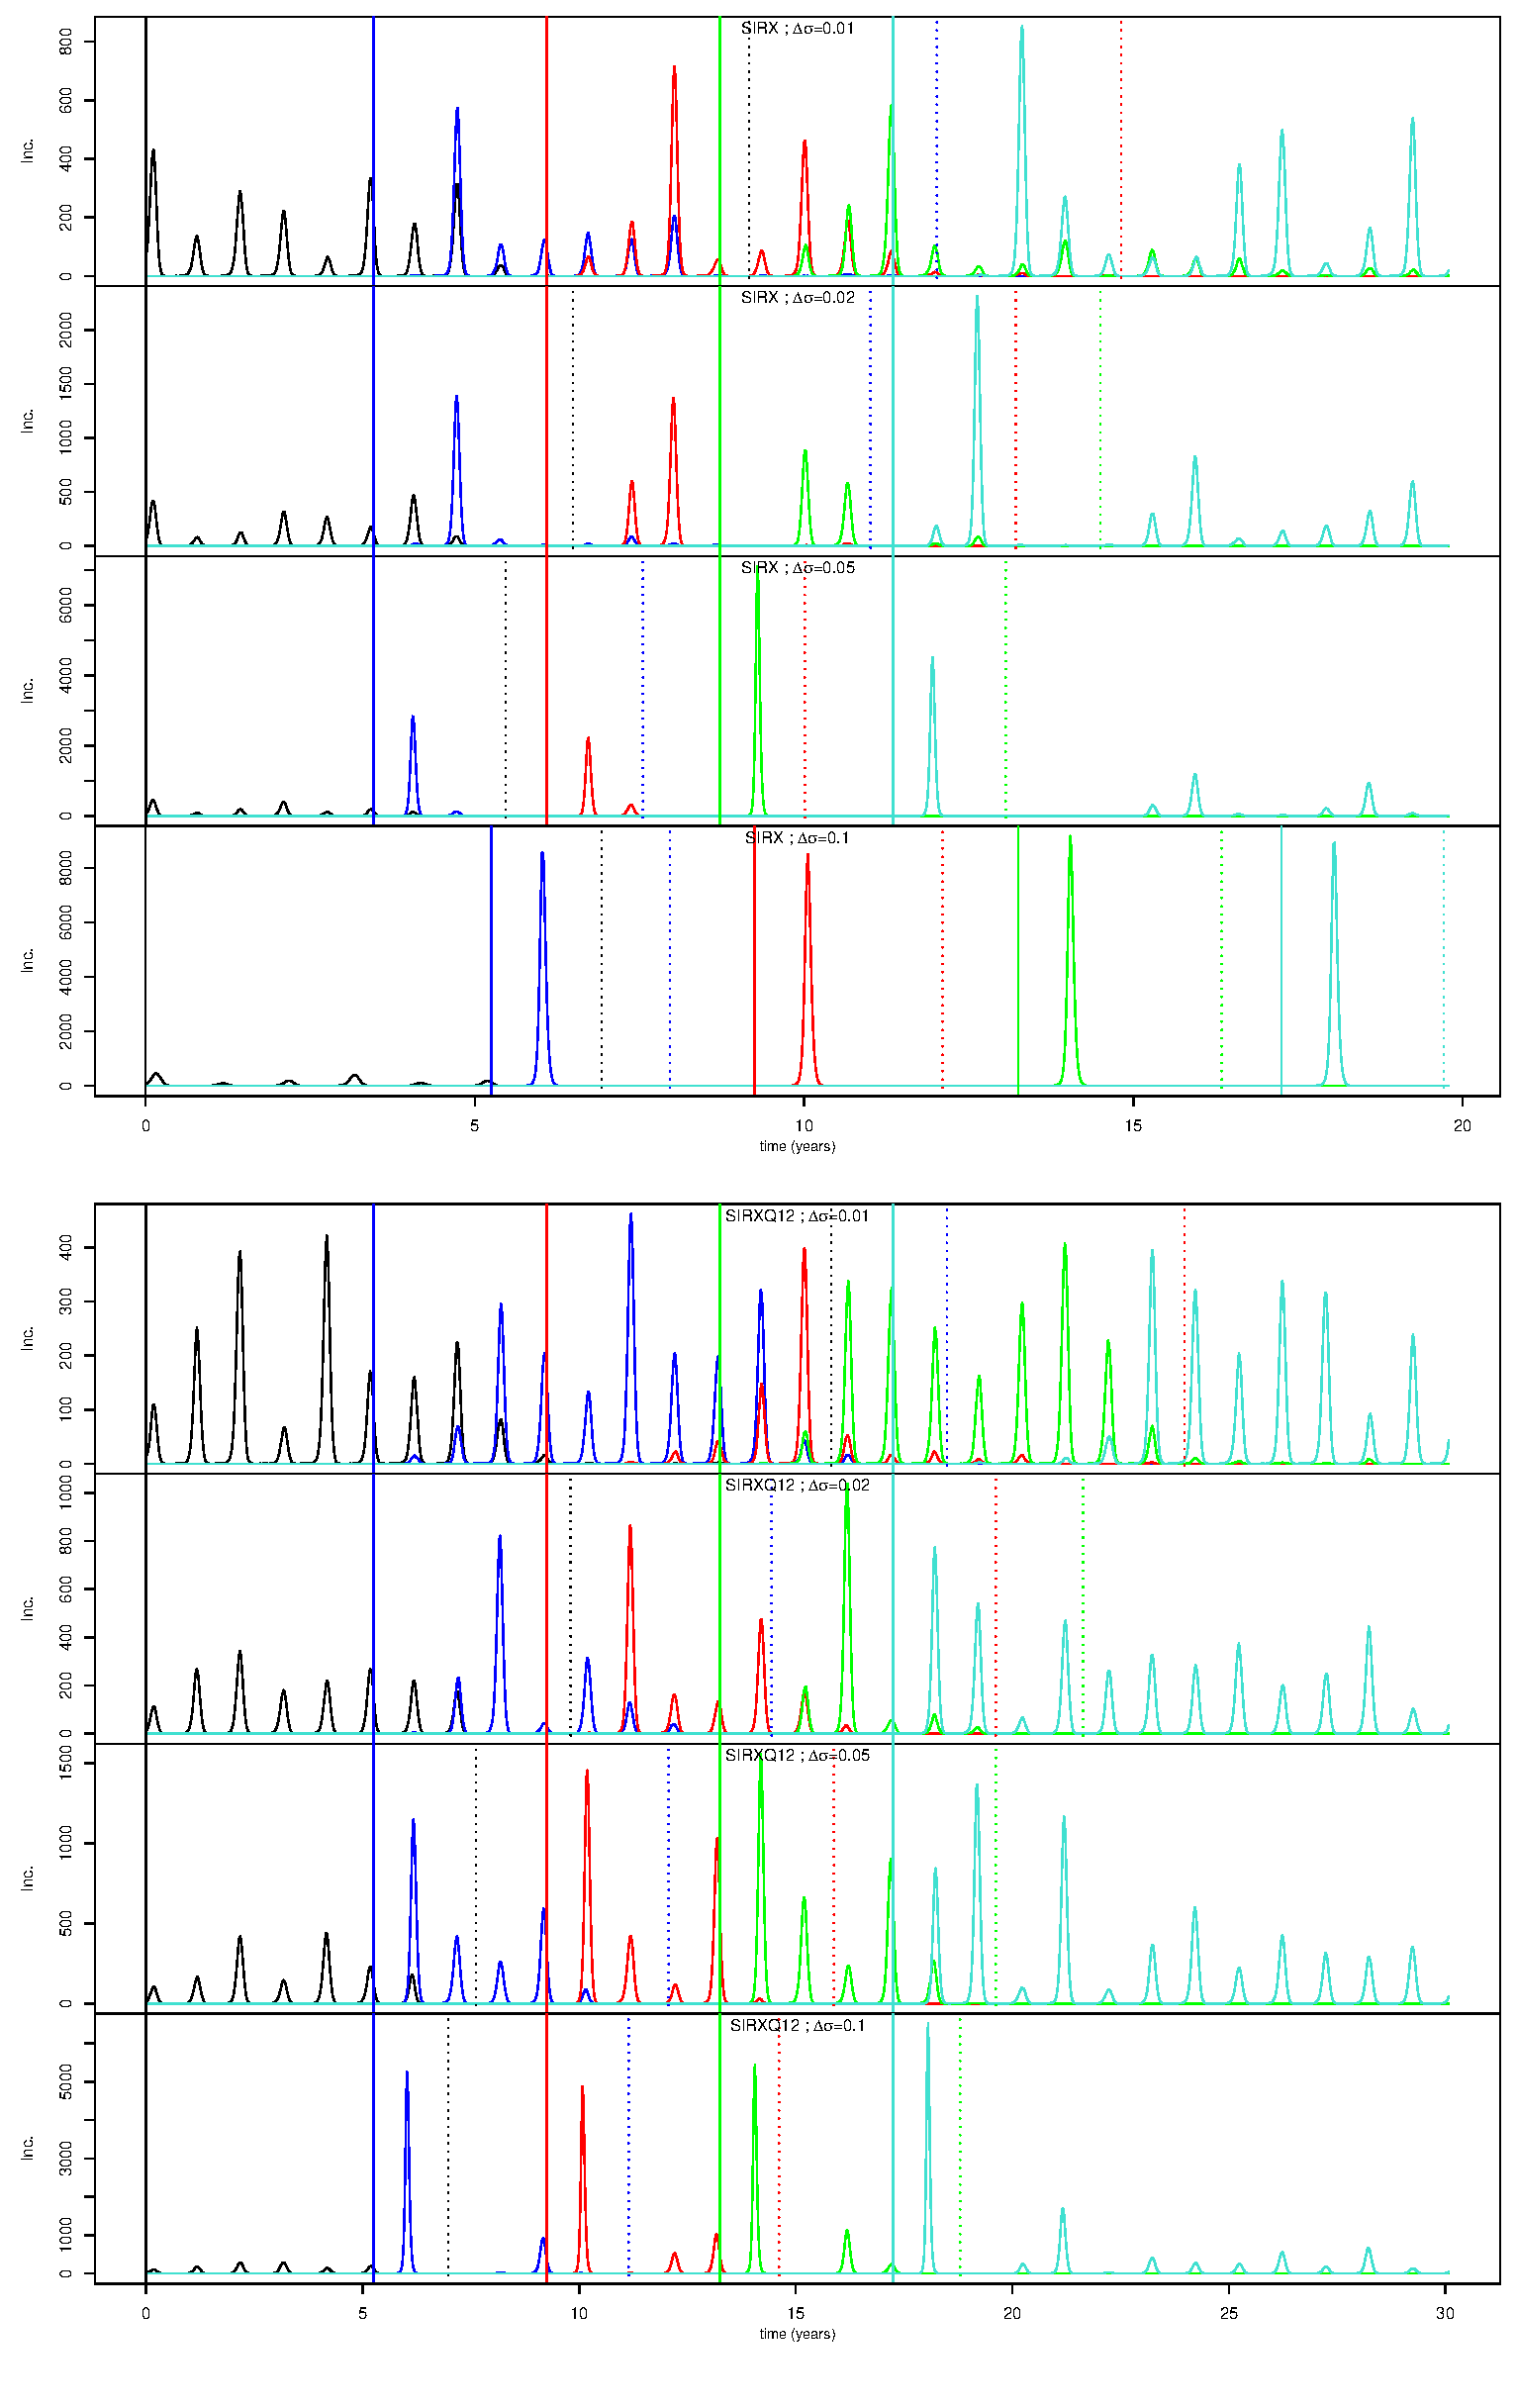
\includegraphics[width=0.8\linewidth]{texte/article3/appendix_diamond/graph/traj_metapop.eps}
  \caption{Typical realisation of the $SIRX$ (first panel) and
    $SIRXQ12$ with immune boosting (second panel) stochastic
    metapopulation models for the city of Paris. First antigenic unit
    is at the endemic equilibrium and the following antigenic units
    are introduced every 4 years in Shenzen on april 1$^{st}$ with an
    initial seed of 100 infected individuals. y-axis is weekly
    incidence per 100 000 inhabitants. Parameters: $\sigma_X=0.3$
    $\Delta\sigma\in\{0.01, 0.02, 0.05, 0.1\}$; $R_0=2$; $1/\nu=4$
    days ; $1/g=1$ year ; $1/q=6$. Vertical plain (dotted) lines are
    introduction (worldwide extinction) times of the antigenic units
    coded by colours. Corresponding annual attack rates are plotted in
    figure~\ref{fig:attack_rate_metapop}, and different realisations
    aggregated by geographics areas in
    figure~\ref{fig:aggreg_metapop}.}
  \label{fig:world_sirx}
\end{figure}



\begin{figure}[!hp]
  \center
  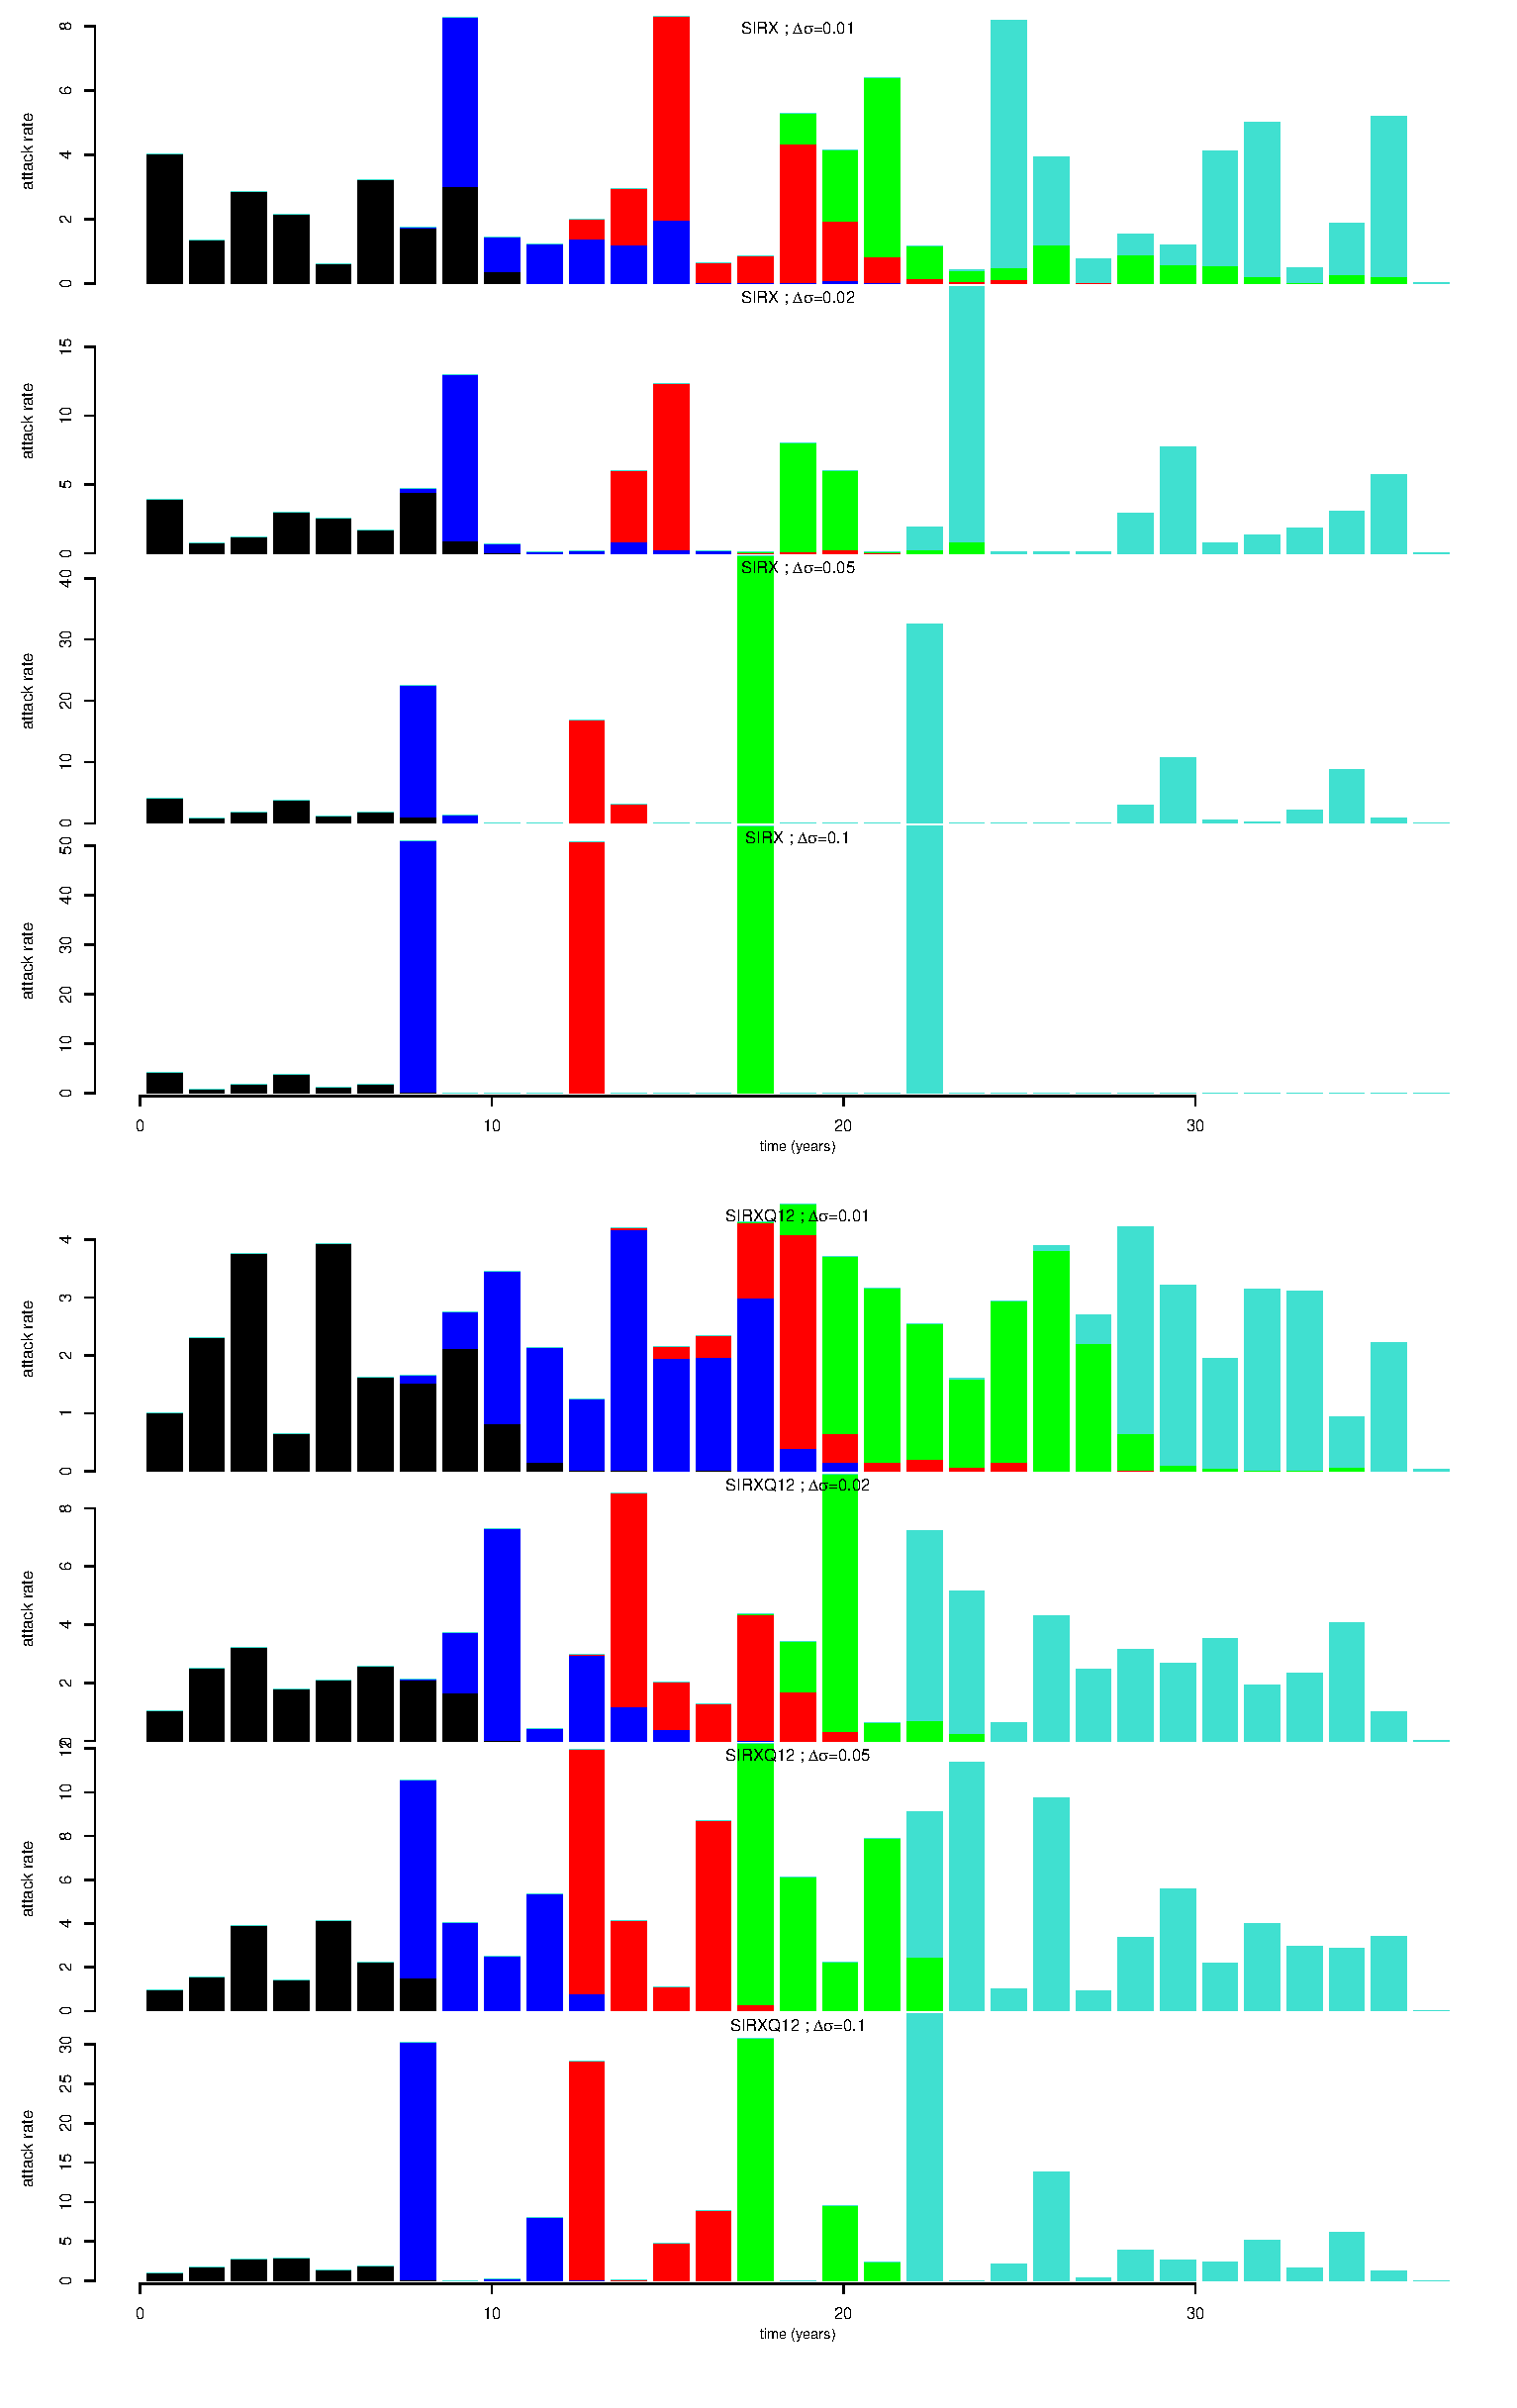
\includegraphics[width=0.9\linewidth]{texte/article3/appendix_diamond/graph/barplot.eps}
  \caption{Evolution of the annual attack rates in Paris for the
    realisations of figure~\ref{fig:world_sirx}.}
  \label{fig:attack_rate_metapop}
\end{figure}



\begin{figure}[!hp]
  \center
  \includegraphics[width=0.9\linewidth]{texte/article3/appendix_diamond/graph/traj5_sirx_siqrx_s03.eps}
  \caption{Trajectories for 20 realisations of the stochastic $SIRX$
    (first panel) and $SIRXQ12$ with immune boosting stochastic
    metapopulation models (second panel) aggregated by world
    areas. First, second and third columns are respectively North,
    Tropics and South. y-axis is weekly incidence per 100 000
    inhabitants. Parameters values are identical to
    figure~\ref{fig:world_sirx} with, for each panel immune escape
    ($\Delta\sigma$) intensities given from top to bottom by $0.01;
    0.02; 0.04; 0.1$. Vertical plain (dotted) lines are introduction
    (worldwide extinction) times of the antigenic units coded by
    colours.}
  \label{fig:aggreg_metapop}
\end{figure}


\begin{figure}[!hp]
  \center
  \includegraphics[width=0.9\linewidth]{texte/article3/appendix_diamond/graph/traj5_sirx_s039.eps}
  \caption{Trajectories for 20 realisations of the stochastic $SIRX$
    (first panel) and $SIRXQ12$ with immune boosting stochastic
    metapopulation models (second panel) aggregated by world
    areas. First, second and third columns are respectively North,
    Tropics and South.y-axis is weekly incidence per 100 000
    inhabitants. Parameters values: $\sigma_X=0.39$
    $\Delta\sigma=0.04$; $R_0=2$; $1/\nu=4$ days ; $1/g=1$ year ;
    $1/q=6$.}
  \label{fig:traj_sirx_s039}
\end{figure}


%\begin{figure}[!hp]
%%  \center
%%  \includegraphics[width=0.8\linewidth]{texte/article3/appendix_diamond/graph/image_sirx.eps}
%  \caption{Per city view of a realisation of the $SIRX$
%    metapopulation model. Black is the resident antigenic unit
%    and red the mutant one introduced in april 1$^{st}$ in
%    Shenzen. City are sorted by starting date of the muntant
%    antigenic unit epidemics and color coded by geographic
%    areas. Parameters values are identical to figure
%    \ref{fig:sirx_s03_039} with $\sigma_X=0.39$.}
%  \label{fig:cooper_sirx}
%\end{figure}
%
%
%\begin{figure}[!hp]
%%  \center
%%  \includegraphics[width=0.8\linewidth]{texte/article3/appendix_diamond/graph/image_siqrx_ferg.eps}
%  \caption{Per city view of a realisation of the $SIRX$
%    metapopulation model. Black is the resident antigenic unit
%    and red the mutant one introduced in april 1$^{st}$ in
%    Shenzen. City are sorted by starting date of the muntant
%    antigenic unit epidemics and color coded by geographic
%    areas. Parameters values are identical to figure
%    \ref{fig:sirx_s03_039} with $\sigma_X=0.39$.}
%  \label{fig:cooper_sirx}
%\end{figure}



%%% Local Variables: 
%%% mode: latex
%%% TeX-master: "../../../phD"
%%% End: 
